%% ****** Start of file aiptemplate.tex ****** %
%%
%%   This file is part of the files in the distribution of AIP substyles for REVTeX4.
%%   Version 4.1 of 9 October 2009.
%%
%
% This is a template for producing documents for use with 
% the REVTEX 4.1 document class and the AIP substyles.
% 
% Copy this file to another name and then work on that file.
% That way, you always have this original template file to use.

%\documentclass[aip,graphicx]{revtex4-1}
%\documentclass[aip,reprint]{revtex4-1}

%\usepackage{graphicx}

%\draft % marks overfull lines with a black rule on the right
%\documentclass[pre,aps,floatfix,authordate1-4,twocolumn]{revtex4-1}
%\documentclass[pre,aps,floatfix,authordate1-4]{revtex4-1}

%\documentclass[aip,jcp,twocolumn]{revtex4}
\documentclass[aip,jcp]{revtex4}
%\documentclass{article}



%\documentclass[aps,prl,preprint,groupedaddress]{revtex4}

\usepackage{rotating} 
\usepackage{times}
\usepackage{graphicx}
\usepackage{setspace}
\usepackage{amsmath}
\usepackage{epstopdf}
\usepackage[obeyFinal]{easy-todo}
\usepackage{csquotes}
\usepackage{mhchem}

%\usepackage{markdown} 

\begin{document}

% Use the \preprint command to place your local institutional report number 
% on the title page in preprint mode.
% Multiple \preprint commands are allowed.
%\preprint{}

\title{Accurate binding of calcium to phospholipid bilayers by effective inclusion of electronic polarization} %Title of paper

% repeat the \author .. \affiliation  etc. as needed
% \email, \thanks, \homepage, \altaffiliation all apply to the current author.
% Explanatory text should go in the []'s, 
% actual e-mail address or url should go in the {}'s for \email and \homepage.
% Please use the appropriate macro for the type of information

% \affiliation command applies to all authors since the last \affiliation command. 
% The \affiliation command should follow the other information.

\author{Josef Melcr}
\author{Hector Martinez-Seara Monne}
\author{Pavel Jungwirth}
\affiliation{Institute of Organic Chemistry and Biochemistry,
Academy of Sciences of the Czech Republic, 
Prague 6, Czech Republic}

\author{O. H. Samuli Ollila}
\email[]{samuli.ollila@helsinki.fi}
%\homepage[]{Your web page}
\affiliation{Institute of Organic Chemistry and Biochemistry,
Academy of Sciences of the Czech Republic, 
Prague 6, Czech Republic}
\affiliation{Institute of Biotechnology, University of Helsinki}


% Collaboration name, if desired (requires use of superscriptaddress option in \documentclass). 
% \noaffiliation is required (may also be used with the \author command).
%\collaboration{}
%\noaffiliation

\date{\today}

\begin{abstract}
% insert abstract here
Classical molecular dynamics simulations give detailed information about membrane structure and dynamics. 
However, there is still a room for improvements in current force fields – it is known from the literature, that the binding of ions, especially cations, to phopholipid membranes is overestimated in all classical models [1]. 
We suggest that the membrane-ion interactions can be corrected by including implicit electronic polarizability into the lipid models through the electronic continuum correction (ECC) [2], which was already applied to monovalent and divalent ions yielding models that feature correct ion pairing [3]. 
Using the electrometer concept [3, 4] and x-ray scattering form factors, our simulations point out that our hypothesis is correct and ECC is indeed a missing important contribution in current classical lipid models. 
Moreover, the solid physical principles behind ECC are found not to hamper other relevant properties of a phospholipid bilayer. 
The new lipid model, "ECClipids", shows accurate binding affinity to sodium and calcium cations and headgroup order parameter response to bound charge. 
We also provide for the first time a realistic stochiometry of bound calcium cations to a POPC membrane, and their binding sites. 
This work will continue as an open collaboration project NMRlipids IV (http://nmrlipids.blogspot.fi).

[1] Catte, A., Girych, M., Javanainen, M., Melcr J., Miettinen, M. S., Oganesyan, V. S. and Ollila H. S.,  PCCP 18(47) 32560-32569 (2016)
[2] Leontyev, I. V., and Stuchebrukhov, A. A., JCTC 6(5) 1498–1508 (2010)
[3] Kohagen, M., Mason, P. E., and Jungwirth, P., J. Phys. Chem. B 120(8) 1454–60 (2015)
[4] Seelig, J., MacDonald, P. M., and Scherer, P. G., Biochemistry 26(24) 7535–7541 (1987)
\end{abstract}

%\pacs{}% insert suggested PACS numbers in braces on next line

\maketitle %\maketitle must follow title, authors, abstract and \pacs

% Body of paper goes here. Use proper sectioning commands. 
% References should be done using the \cite, \ref, and \label commands


% Here I write pseudo-article statements that will make the main argument.
% Beautiful polished sentences will be formed only afte we agree on these basic things
\textbf{General Introduction}

 motivation, significance of membranes, phospholipids and simulation.

 assumptions (so that we have structure of the paper like in a mathematical proof) -- 
 MD simulation is a good tool for studying molecules.
 classical MD models can describe lipids accurately, 

 MD is ... and it serves ... it is useful for ... (describe throuhg references)

 Lipid membranes, especially phospholipid membranes; their significance for life, sciences, society, pharma ...

\textbf{Specific introduction: current FFs and MDEC/ECC}

 Current force fields -- pros and cons, at a good shape in many aspects, agree on various properties.  -- write basic ideas from the lipid-FF whitepaper I did recently.

 lipid force fields fail in description of membrane-cation interaction -- could be answered by ECC? 
Cations were shown to generally overbind in PC lipid bilayers in NMRlipids II project. 
Here we propose that the cation overbinding can be corrected by implicitly inducing electronic polarizability in lipid headgroups by scaling the partial charges -- i.e. MDEC/ECC~\cite{Leontyev2015}\todo{Bulid BibTex references database.} paradigm.

MDEC -- or -- ECC 
\todoii{choose one}{We have to decide whether we will refer to the method as a correction (ECC) or as a MD simulation paradigm (MDEC) -- and choose on of these labels. -- Joe: use ECC as we apply MDEC rather as a correction to current state not as a new paradigm for FF development.}
MD in electronic continuum as in \cite{Leontyev2015} or electronic continuum correction as in \cite{Jungwirth2015}

Describe ECC: good physical concept for treating part of the polarizability (electronic) in a simple mean-field way.

Succesful application: Works for cations \cite{Jungwirth2015,Kohagen..}\todoii{REF}{Missing references} -- motivation for its application to zwitterionic lipids like POPC.

Hypothesis: ECC helps in describing even zwitterionic molecules like POPC, will be demonstrated through headgroup order parameter response to cationic molecules.

\textbf{Main body starts:}

ECC and solvation $\Delta G$.(from \cite{Leontyev2015} \todoi{Pavel: do not replicate Stuchebrukhov paper, write it very briefly}: hydration $\Delta  G_{hyd}$ can provide good structure and energetics, but will fail in good interactions -- already proved for cations)
In addition, $\Delta G_{hyd}$ -- the usual target for parametrization of small molecules in classical force fields -- is not the right target in the MDEC/ECC paradigm -- part of $\Delta G = \Delta G_{nuc} + \Delta G_{el}$ is already included in the polarization of electrons, and only the remining part of $\Delta G$,  $\Delta G_{nuc}$, belongs to the polarization of the nuclei. 
Hence it is non trivial, how large should be the scaling factor $f_\sigma$ -- it should lay between $1$ and $f_q$, the limits for the original interaction energy and its limit when we neglect the $\Delta G_{el}$ term in $\Delta G_{hyd}$. 

How do I apply ECC on Lipid14 POPC and why such choice (i.e. $f_\sigma$, $f_q$ and definition of the scaled region).
Region definition: headgroup requires optimization, tails appear already accurate enough. 
Choice of $f_q$: value 0.8 reflects the fact that the charges in Lipid14 were derived in vacuum, whereas they should rather be the average of vacuum and solvated charges (so called IPolQ charges \cite{Cerutti2013}, both charge-sets can be taken from \cite{Maciejewski2014a}). 

why did I choose Lipid 14 -- good ratio of $\alpha / \beta$ response~\cite{NMRlipid2paper}.

\textbf{Observations, how does the system behave, what are its macroscopic properties:}

Accurate binding of \ce{Na^+} and \ce{Ca^{2+}} cations. 

Accurate electrometer response to \ce{Na^+}, \ce{Ca^{2+}} and \ce{DHMDMAB} cationic surfactant. 

What affects the headgroup OP response?: The response of the headgroup order parameters is improved both through diminished affinity towards the cations and through lower headgroup response to the bound charge (from simulations with \ce{DHMDMAB} surfactant). 
The responses of headgroup OPs are shown in Fig. \ref{OrderParameterCHANGESnewMODELS}. 

Gives correct scattering form factor -- reliable structural properties (especially in combination with OPs) and good ground for interpretting experimental data.

Provides/predicts correct stoichiometry for \ce{Na^+}, \ce{Ca^{2+}} and their interaction energies with the lipid membrane.
Samuli: the main selling argument would be that we solve the details (stoichiometry, coordination numbers, etc.) of cation binding in PC bilayer. 

Preserves other relevant properties: APL, Order Parameters (OPs of headgroup and tails), 
diffusion? \todoi{diffusion can be even improved -- and doesn't have to. We may as well omit it.}, 
elasticity? \todoi{check elastic properties -- do they change, improve, worsen?? -- likely not crucial for the main message of the paper.} 
-- however, it is still garbage in-garbage out

The glycerol backbone and headgroup order parameters are plotted in
Fig \ref{HGopsNEWmodels.eps} for reference models and EEC models. The difference,
i.e. the effect of scaling on these parameters, is shown in Fig. \ref{HGopsNEWmodelsCHANGE}.

\begin{table}
  \caption{Area per lipid from different models for POPC without ions\label{apls} }
  \begin{tabular}{c c c}
    model          & A (Å$^2$)   & Temperature [K] \\
    \hline
    Lipid14 (literature)  & 65.6$\pm$ 0.5  &  303 \\
    Lipid14ecc0.80+sigma0.875 &        &  313    \\
    GMX small patch           & 64.9   &         \\
    GMX 4xbig patch           & 65.5   &         \\
    oMM small patch           & 63.65  &         \\
    oMM 4xbig patch           & 63.7   &         \\
    \hline
    experiment \cite{Jambeck2012}\todoii{REF}{put original references, not Slipids param. paper.}  & 62.7  &  293    \\
    experiment  & 64.3  &  303    \\
    experiment  & 67.3  &  323    \\
    experiment  & 68.1  &  333    \\
    experiment POPE  & 56.6 &  303    \\
    \hline
  \end{tabular}
\end{table}

\textbf{Required figures}

- Figure showing the system: POPC, membrane, atoms involved in headgroup OPs.\todoi{This is probably sufficient as the last thing we would do -- and will probably provide a good basis for TOC graphic.}

- Figure comparing order parameters (Fig.~\ref{HGopsNEWmodels}) and form factor \todoi{The original L14 form-f are worse than those in the L14 paper -- I'd better double check it and make sure I use the same settings and version for all simulations consistently for a good comparison.}between original Lipid14, new model and experiments,

\begin{figure}[]
  \centering
  \includegraphics[width=9.0cm,angle=-90]{../Fig/form-f_exp-l14-eccl17.eps}
  \caption{\label{fig:form-f}
    X-ray scattering form factors from experiments~\cite{Kucerka2011} and simulations using Lipid14 and ECCLipids17 models.  }
\end{figure}

\begin{figure}[]
  \centering
  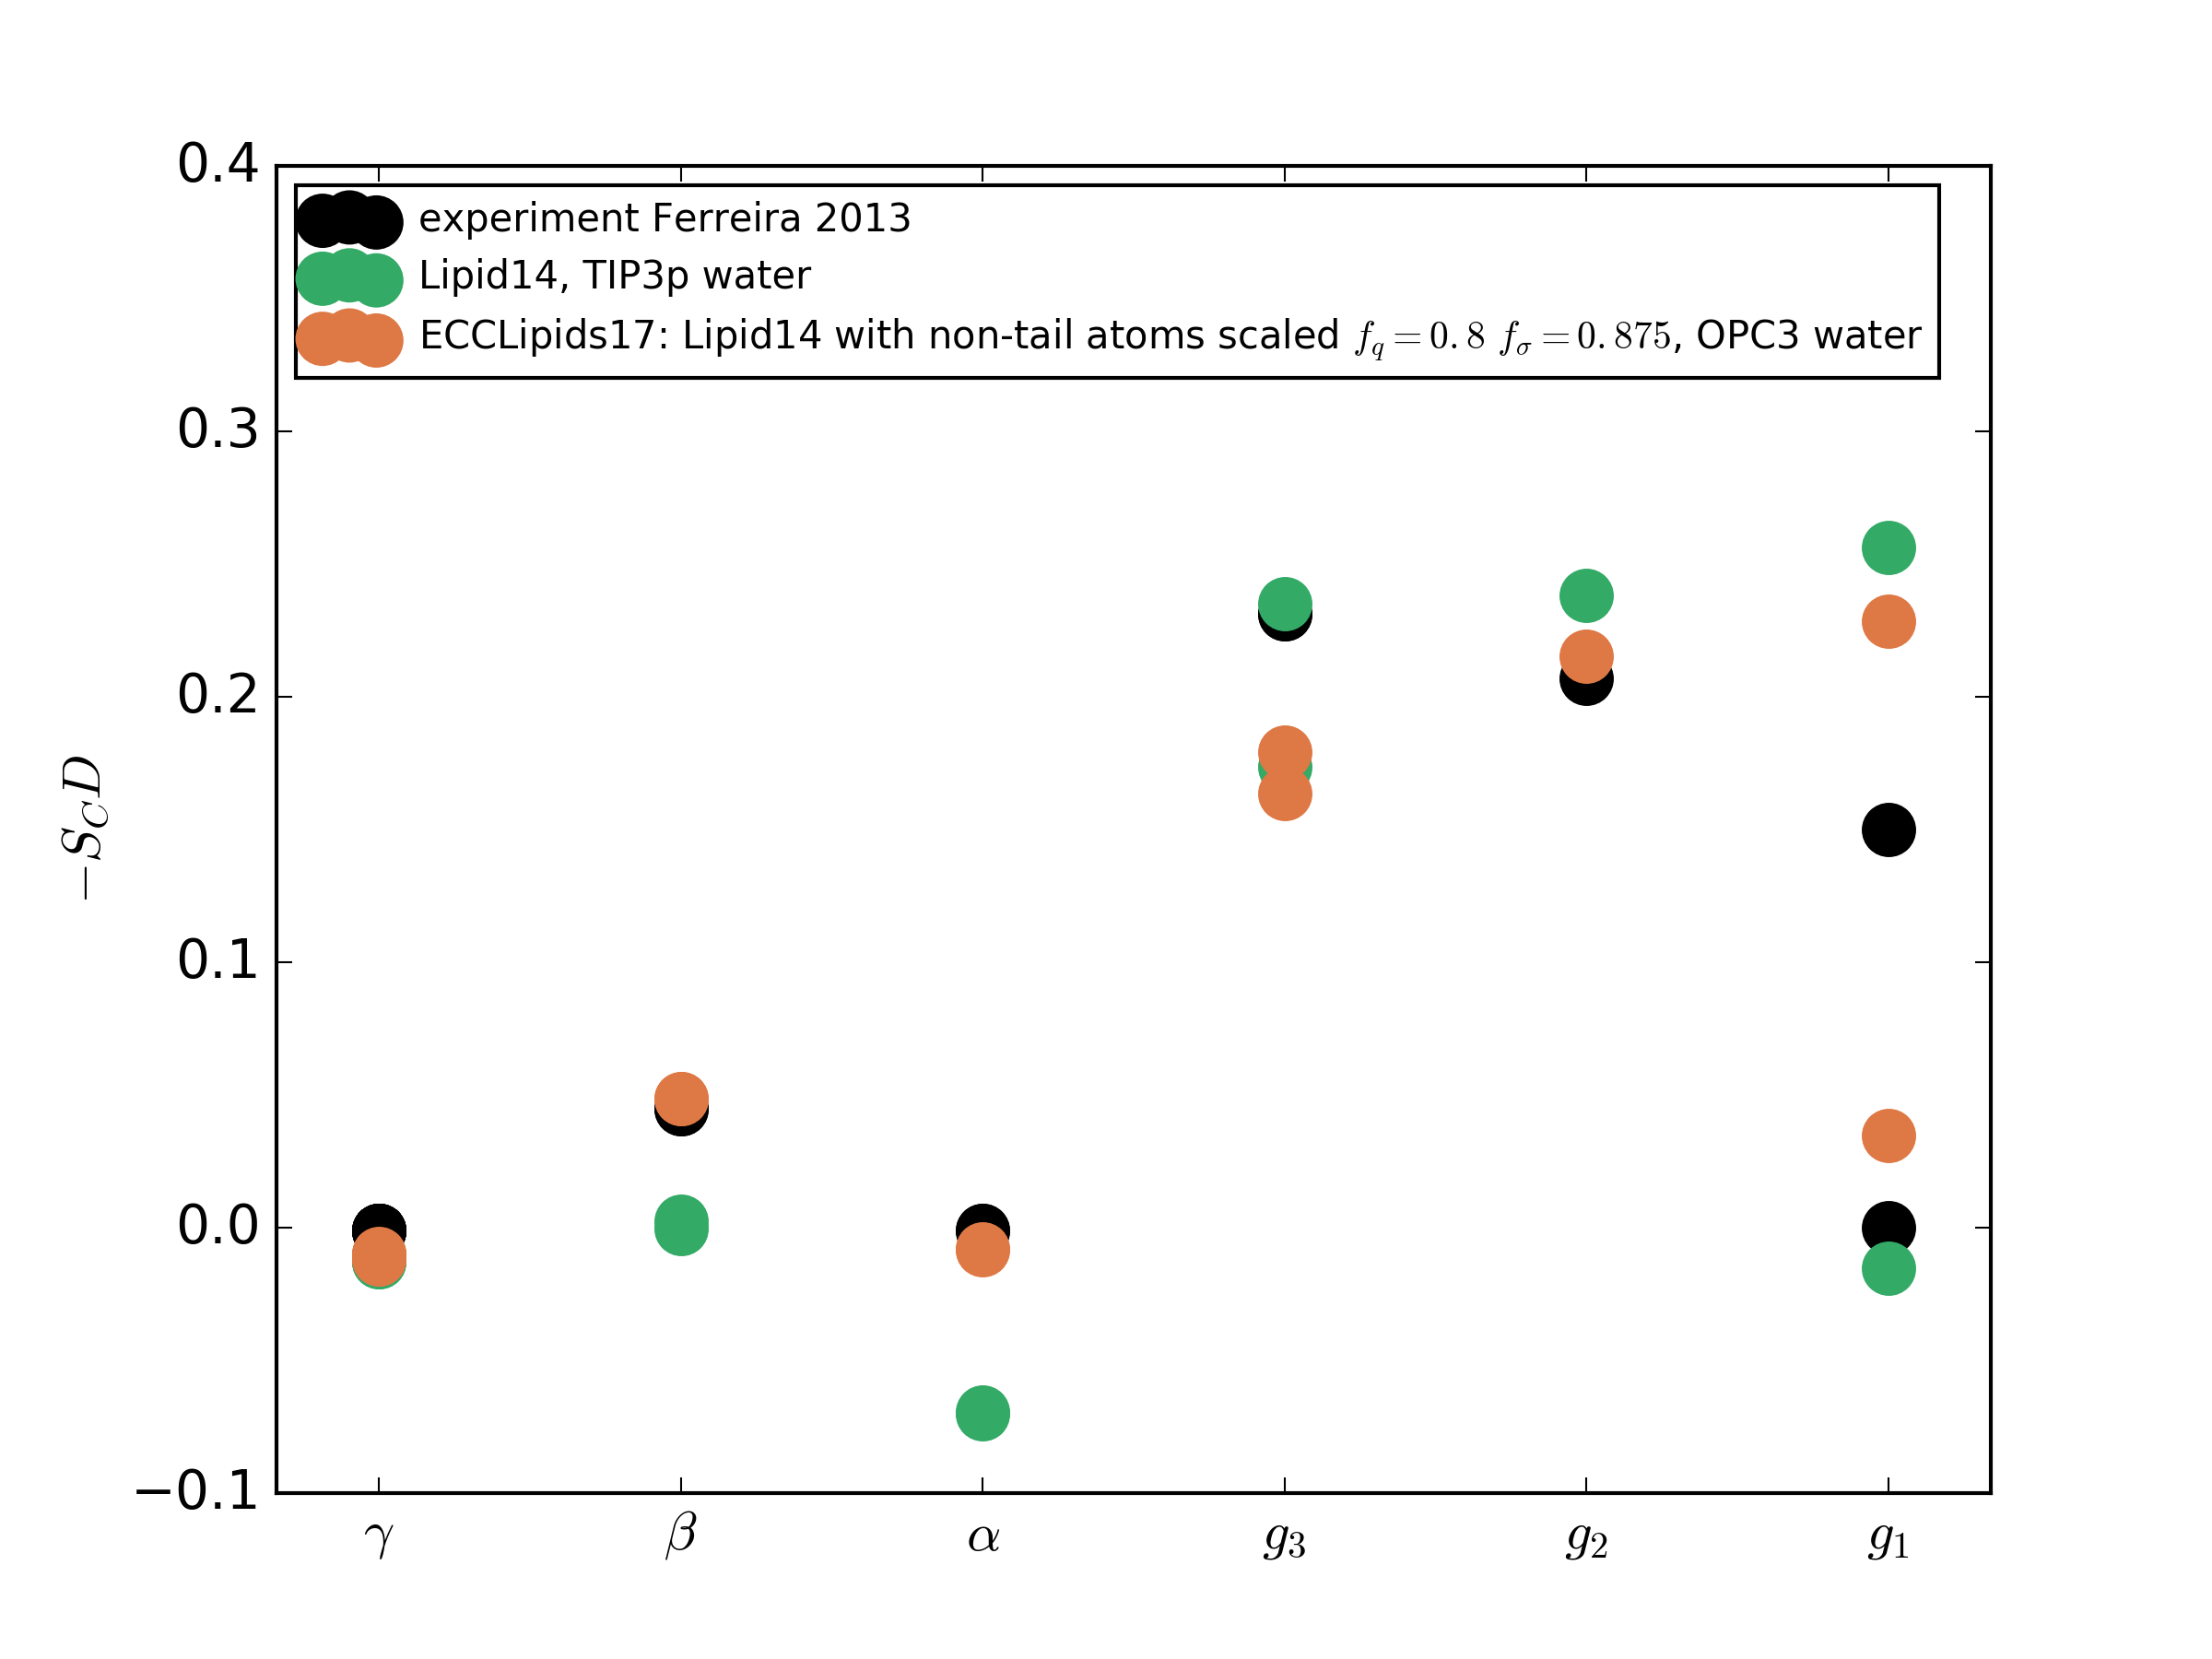
\includegraphics[width=9.0cm]{../Fig/ipython_nb/Headgr_OPs_exp-L14-ECCL17.png}
  \caption{\label{HGopsNEWmodels}
    Headgroup and glycerol backbone order parameters from standard Lipid14 and EECLipid17 models.}
\end{figure}


- Figure showing order parameters as a function of \ce{NaCl} and \ce{CaCl_2} concentrations~
\todoii{ongoing}{Actual concentration of cations in simulation has yet to be estimated. 
If it varies too much from the nominal concentration, I may need to tweak the scaling factors, $f_q$ or only $f_\sigma$, to accomodate it. 
However, it is very unlikely, response to the surfactant \ce{DHMDMAB} is OK. 
Big patches with loads of solvent are running at the moment to guide me on the possible finite-size errors and this conc-error.} 
from Lipid14, new model and experiments (like current Fig. 1, but only original and final models)

\begin{figure}[]
  \centering
  \includegraphics[width=16.0cm]{../Fig/OrdParChanges_NaCl_CaCl2_surf.eps}
  \caption{\label{OrderParameterCHANGESnewMODELS}
    Headgroup order parameter changes as a function of concentration of cations or cationic surfactant DHMDMAB. }
\end{figure}

- Figure(s) analysing binding details (density profiles, lipids bound per ion, something else?).

\begin{figure}[]
  \centering
  \includegraphics[width=9.0cm,angle=0]{../Fig/CAdensities.eps}
  \caption{\label{fig:cacl-dens}
    Density profiles of \ce{Ca^{2+}} and \ce{Cl^-} for Lipid14 model with Aquist parameters and with ECC ions and ECCLipids17 with ECC ions. }
\end{figure}


\textbf{Discussion:}

other lipids: charged lipids? -- ongoing research in our lab.
I'm currently working on POPE with Aniket for curved (and flat) membranes. 

Samuli: From the point of view of this paper, the most relevant other lipid to study would be DPPC to see if we can reproduce the difference between POPC and DPPC in experiments.

Joe: In addition, there are more experimental OP data on DPPC. However, it is not necessary and we can leave it to the community project. 

Role of water model: we use OPC3 (current best), it would be worth giving an estimate how results change when we use say SPCE or even TIP3p at least in the SI (so that the reader knows what errors to expect comming from these sub-optimal models). 
In addition, there is protein force field Amber15-FB, which uses water close to OPC3, TIP3pFB \todoii{REFs}{add references here}.

questionable charge distribution from RESP -- a leeway for further tweaks of the FF.
It is not obvious that RESP charges provide the best description, especially due to its non-uniqe solution. 
Shall we solve RESP fitting with the constraint of full charges and then scale down, or shall we rather solve the fitting with a scaled total charge target?

acheivable accuracy of the MD engines themselves (mainly Hector's worry) is another limiting factor in fine tuning parameters -- solid physical ground helps.

application of the correction to other lipid models: The rule looks general, however, it depends on how accurate the original model was.
From preliminary simulations with POPE, it looks that the rule works for Lipid14 FF, at least for zwitterionic headgroups.

\textbf{Conclusion:}

Reiterate what we did...

This will be a foundation stone of a new open-collaboration project NPRlipid 6 in nmrlipids.blogspot.fi....
















% Tables may be be put in the text as floats.
% Here is an example of the general form of a table:
% Fill in the caption in the braces of the \caption{} command. Put the label
% that you will use with \ref{} command in the braces of the \label{} command.
% Insert the column specifiers (l, r, c, d, etc.) in the empty braces of the
% \begin{tabular}{} command.
%
% \begin{table}
% \caption{\label{} }
% \begin{tabular}{}
% \end{tabular}
% \end{table}

% If you have acknowledgments, this puts in the proper section head.
\begin{acknowledgments}
% Put your acknowledgments here.
\end{acknowledgments}
\newpage
\appendix
\begin{center}
{\bf SUPPLEMENTARY INFORMATION}
\end{center}


% Create the reference section using BibTe
\bibliography{refs.bib}

%\newpage
%\section{APPENDIX: The NMR results reported by Tiago Ferreira}

\listoftodos

\end{document}
%
% ****** End of file aiptemplate.tex ******
